\chapter{DNS}
\label{chp:dns}

\section{Introduction}

\Gls{dns} is an important part for the internet. It was designed and standardized in the mid and late 1980s as the previous system \texttt{HOST.TXT} was headed for and encountering problems \cite{Mockapetris:1988:DDN:52324.52338}, but has since been updated and configured many times. \Gls{dns} needed to be able maintain a fast response time as the database grew larger, this was solved by using a hierarchical set up. This means that each layer only has a limited information and sends the request to a new server until it reaches the correct server, called \texttt{name server}. It started with one root server, which has expanded to 13 today. The each layer of the hierarchy is called a zone, and it delegates the responsibility for underlying zones delimited by the \texttt{dot} in the request name.

When a request for \texttt{ntnu.no} goes through \Gls{dns} it starts in the root zone, where it sent down the hierarchy to the \texttt{.no} zone.
% Here is the information about the name server for \texttt{ntnu.no} which again is one zone lower. This name server sends the request to the name server for \texttt{ns1.} which then replies.

\begin{figure}
\centering
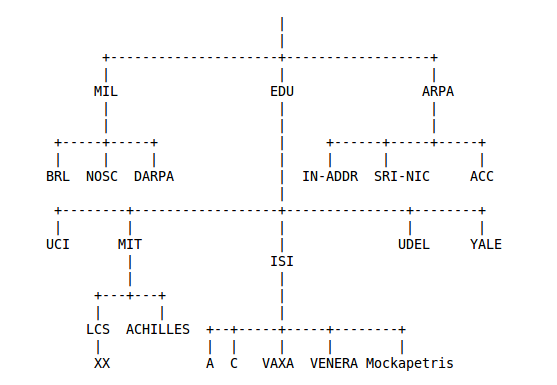
\includegraphics[scale=0.5]{figs/namespace_example.png}
\label{fig:namespace}
\caption{Example of name spaces of a root with MIL, EDU and ARPA as immediate subdomains. Each leaf is a domain \citep{mockapetris1987domain}.}
\end{figure}



consists of many distributed databases 
The main function of \Gls{dns} is to translate domain names to IP addresses. 

 mostly used to translate a domain name to an IP address which the network use to route http traffic


This type of lookup receive an \texttt{'A'} record if the IP is an ipv4 address and \texttt{'AAAA'} if it's an ipv6 address. \texttt{'CNAME'} is also a much used response. it returns the correct domain name for the 'A' lookup, e.g. if you want to go to aftenposten.no, you could write ap.no the \Gls{dns} then respond with a CNAME response containing aftenposten.no which automatically trigger a new request for aftenposten.no which give an 'A' response containing the ipv4 address. There are over 30 different record types in the \Gls{dns}. Every one has their different purpose and therefore different maximum size on the payload. \Gls{dns} mostly use UDP on port 53, but could also use TCP on the same port. TCP is used when the payload is over 512 bytes or if there is a zone transfer. 

\Gls{dns} is build as a hierarchical system where each level sends you along until you have reached the correct server. The internet has 13 root servers, and a lookup in the system is backwards. The easiest way to explain this is with an example. If you request \texttt{some.test.example.com} the first request will be to the root server which will look up the IP-address of the server that controls the .com domain. Next the .com server looks up who controls the example.com domain, and the example.com server finds the \Gls{dns} server of test.example.com. At last the test.example.com \Gls{dns} server returns the IP-address of some.test.example.com. Since this process takes a long time, most responses has a \Gls{ttl} which is how long the router should use the given IP-address as a response to requests for that domain.

Normally a \Gls{dns} server in an enterprise does not send requests directly to the internet, but use an internal \Gls{dns} server instead. If you are the owner of the authoritative server for a domain, you can control the responses. This is what a \Gls{dns} tunnel exploits, which will be explained more in the next section. 





 